%%%%%%%%%%%%%%%%%%%%%%%%%%%%%%%%%%%%%%%%%%%%%%%%%%%%%%%%%%%%%%%%%%%%%%%%%%%%%%%
% Active Learning Machine Learning Methodology %%%%%%%%%%%%%%%%%%%%%%%%%%%%%%%%
% %%%%%%%%%%%%%%%%%%%%%%%%%%%%%%%%%%%%%%%%%%%%%%%%%%%%%%%%%%%%%%%%%%%%%%%%%%%%%
%
% Points to mention:
%    Voronoi is used because it is insensitive to volume expansions of structure
%    TODO: Explain PCA analysis
%    TODO: Get PCA reference
%
% TODO:
%    Why AB2 and AB3
%%%%%%%%%%%%%%%%%%%%%%%%%%%%%%%%%%%%%%%%%%%%%%%%%%%%%%%%%%%%%%%%%%%%%%%%%%%%%%%


% ################################# Paragraph #################################
% %%%%%%%%%%%%%%%%%%%%%%%%%%%%%%%%%%%%%%%%%%%%%%%%%%%%%%%%%%%%%%%%%%%%%%%%%%%%%
% General intro to AL scheme
% Basic gist, i.e. define our candidate space of materials to explore within
% (we do this by looking taking all structurally unique systems in DBs)
% To start the AL we take the few systems that have DFT calcs (more generally
% we can just choose random structures)
% We then build a surrogate model (GP, initially really bad) to predict the
% stability of the entire candidate space
% %%%%%%%%%%%%%%%%%%%%%%%%%%%%%%%%%%%%%%%%%%%%%%%%%%%%%%%%%%%%%%%%%%%%%%%%%%%%%
% | - Paragraph start
% Maybe "crystal structures" instead of "materials"? More to the point?
%CP: agree
Here, we present a machine-learning based methodology for discovering new stable and meta-stable crystal structures.
%
Our approach builds on the principles of surrogate active learning [Refs?],
where a model is iteratively trained on available DFT data.
%
The model predictions are used as a surrogate to the DFT energy evaluations,
which are used to acquire new systems for DFT in the population based on an acquisition criteria.
% Add the Hammer paper (R58) as another citation
Active learning in conjunction with genetic algorithms has been demonstrated to successfully speed up materials discovery for alloy nanoparticles \cite{Jennings2019}, and ...[Other refs?],  structural optimizations \cite{hansen2019atomistic}, and transition-state calculations \cite{torres2019low}.
% TEMP
The methodology consists of two steps (outlined in  \ref{fig:all_diagram}).
%
The first step is the generation of the candidate space,
which defines the inclusive list of all crystal structures to be screened through during the search routine.
%
Since the initial candidates determines which structures that can ultimately be discovered, it is crucial to define a candidate space that is sufficiently diverse.
% TEMP Say more
The second part of the algorithm is the iterative active learning algorithm.

% | - __old__
% Our machine learning accelerated materials discovery method proceeds through the following steps:
% First, the dataset of candidate materials is constructed.
% This data set will define the totality of materials that will be considered by the search algorithm,
% this is done because the search space of materials is not a continous space but a discrite array of individual structures.
% Next, the dataset of materials is transformed into a vectorial representation by using a fingerprinting method that encodes the relevent chemical and structural information.
% __|

% __|


% ################################# Paragraph #################################
% %%%%%%%%%%%%%%%%%%%%%%%%%%%%%%%%%%%%%%%%%%%%%%%%%%%%%%%%%%%%%%%%%%%%%%%%%%%%%
%
% %%%%%%%%%%%%%%%%%%%%%%%%%%%%%%%%%%%%%%%%%%%%%%%%%%%%%%%%%%%%%%%%%%%%%%%%%%%%%
% | - Paragraph start
% TODO Ask @Ankit for these numbers
% The MP project number should be correct, but the OQMD number might be wrong
% MP{AB2: 3995, AB3: 2849} | OQMD{AB2: 533, AB3:20915}
In Schema \ref{fig:all_diagram} we show the {\bf overall process with the integrated active learning loop}. {\bf We start with ...}.
%
{\bf We continue with  with XXX...}
%
The structures that comprise the candidate data sets for \IrOtwo and \IrOthree were constructed by parsing for all bulk \ABtwo and \ABthree structures in both the Materials Project\cite{Jain2013} and OQMD\cite{Kirklin2015} databases
(in total 4528 \ABtwo and 23764 \ABthree entries).
%
Structurally redundant systems were then removed via a space-group based structural classification scheme developed by Jain et al. \cite{Jain2018}.
%
The resulting data set is composed of 697 \ABtwo and 259 \ABthree structural prototypes for which iridium and oxygen were replaced for the A and B sites, respectively.
%
Finally, a coarse isotropic volume relaxation was performed to accommodate for the difference in atomic radii of Ir and O to the elements that originally comprised the structure in OQMD/MP.
%
Additional details about our method can be found in the SI.
% TODO Double check numbers
Only candidates that were successfully optimized with DFT were ultimately included so that the model could be properly validated,
which gives a final candidate data set of 448 and 258 \ABtwo and \ABthree structurally unique polymorphs.
%
While size of this dataset is not particularly large, it will serve the purpose of demonstrating the polymorph discovery routine as a proof of concept.
%
Additionally, the dataset is small enough that computing all of the structural candidats with {\it ab-initio} DFT is tractable, thus allowing us to validate the performance of the model.
% __|


% ################################# Paragraph #################################
% %%%%%%%%%%%%%%%%%%%%%%%%%%%%%%%%%%%%%%%%%%%%%%%%%%%%%%%%%%%%%%%%%%%%%%%%%%%%%
%
% %%%%%%%%%%%%%%%%%%%%%%%%%%%%%%%%%%%%%%%%%%%%%%%%%%%%%%%%%%%%%%%%%%%%%%%%%%%%%
% | - Paragraph start
The candidate data set was featurized using the Voronoi tessellation fingerprinting scheme developed by Ward et al. \cite{Ward2017} which produces a 271 feature vector for each material that are insensitive to isotropic expansions and contractions in a crystals lattice.
% How many columns of the 271 are redundant if stoich and composition are frozen
Herein, we apply our active learning model to the \IrOtwo and \IrOthree spaces separately, because we are interested in the most stable polymorphs at each stoichiometry. Constraining the candidate space to having uniform stoichiometry reduces the 271 feature vector to 101 non-zero variance features, thus reducing the dimensionality of our problem significantly.
% COMBAK
Further dimensionality reduction is achieved via a principle component analysis (PCA) \cite{Tipping1999}, which was used to reduce the remaining 101 features to 11.
%
The active learning algorithm proceeds through iterative generations of ML training, prediction, and acquisition steps that are visualized in figure \ref{fig:iro2_al}.
% COMBAK Did I get all of the important features of GP here? @Jose
To start, Gaussian process (GP) regression is used to train a regression model on a small seed set of DFT formation energies from randomly selected structures in the candidate space.
%
The model is then used to predict the formation energies of the entire candidate space.
%
Following this, the predictions are used to determine which systems to acquire, by minimizing the so-called GP-UCB acquisition function:
% The name for this kind of acquisition is calld GP-UCB (Upper confidence bound)
% https://www.cse.wustl.edu/~garnett/cse515t/spring_2015/files/lecture_notes/12.pdf
\begin{equation}
    U = \mu - \kappa \sigma,
\end{equation}
%
where $\mu$ and $\sigma$ is the predicted mean and standard deviation of the formation energy,
and $\kappa$ is a free parameter to tune the relative weighting between exploiting low formation energy systems (small $\kappa$) and exploring high uncertainty regions of the candidate space (large $\kappa$).
%
In this work we attempt to trade off exploitation and exploration by weighting the predicted formation energy and the associated uncertainty to bias systems that are both low energy and high uncertainty.
%
Here, $\kappa$ is set to $1$ which equally weights the energy and uncertainty.
% TODO N is used into mean number of atoms (FIX)
Once ranked, the N systems that minimize the acquisition function are selected for full DFT calculations, which are included in the training data of subsequent AL generations.
% COMBAK We are discussing alternative convergence criteria, or whether to even
% have convergence criteria here
The AL loop proceeds until convergence is achieved, which here is chosen to be the generation at which the structures within the range of metastability, here taken as 0.1 eV/atom, are unchanging over three consecutive generations.
% __|



% | - Figure | Active Learning Algorithm **************************************
\begin{figure*}[!htb]
\centering
\makebox[\textwidth][c]{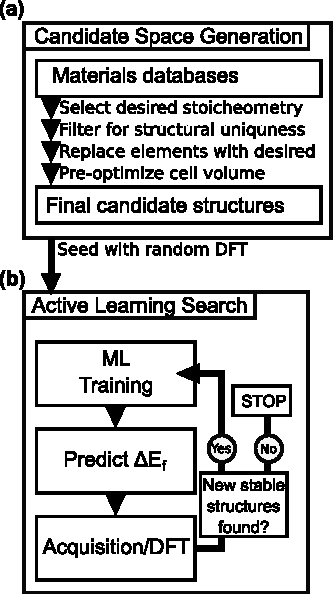
\includegraphics
  {02_figures/al_diagram/Surrogate_model_mine.pdf}
  }
\caption{\label{fig:all_diagram}
% Probably better to keep this caption really concise and refer to the text
Process flow diagram for the active learning accelerated algorithm. The procedure is composed of (a) generation of the candidate set of considered crystal structures constructed from DFT materials databases and (b) iterative active learning surrogate search of the candidate space.
}
\end{figure*}
% __|
